\documentclass{article}

\usepackage{fullpage}

\usepackage{amsmath}
\usepackage{amsfonts}
\usepackage{bbm}



\usepackage{xcolor}
\newcommand{\jarad}[1]{{\color{red} #1}}


\usepackage{tikz}
\usetikzlibrary{arrows.meta,positioning}

\usepackage{natbib}
\bibliographystyle{abbrvnat}
\setcitestyle{authoryear,open={(},close={)}}

\newcommand{\ind}{\stackrel{ind}{\sim}}
\newcommand{\1}{\mathbbm{1}}
\newcommand{\nug}{nug}

\begin{document}



\section{Gaussian Process}

\subsection{Scalar GP}

Let $Y\sim GP_{\mathbb{R}^{D}}(m,k)$ indicate a scalar Gaussian process (GP),
i.e. $Y\in \mathbb{R}$,
such that for any collection of locations $x_1,\ldots,x_N \in \mathbb{R}^{D}$,
$D \in \mathbb{N}$,
we have
\[
\left[ \begin{array}{c} Y(x_1) \\ \vdots \\ Y(x_N) \end{array}  \right] \sim
N\left(\left[\begin{array}{c}
m(x_1) \\ \vdots \\ m(x_N)
\end{array} \right],
\left[ \begin{array}{ccc}
k^{\nug}(x_1,x_1) & \cdots & k^{\nug}(x_1,x_N) \\
\vdots & \ddots & \vdots \\
k^{\nug}(x_N,x_1) & \cdots & k^{\nug}(x_N,x_N)
\end{array} \right] \right)
\]
with mean function $m: \mathbb{R}^{D} \to \mathbb{R}$ and
covariance function $k: \mathbb{R}^{D}\times \mathbb{R}^{D} \to \mathbb{R}$.
A general form for the covariance function is
\[
k^{\nug}(x,x') = k(x,x') + \tau^2\1(x=x'), \quad
k(x,x')  = \sigma^2 k^{cor}(x,x')
\]
for a nugget-less covariance function
$k: \mathbb{R}^{D}\times \mathbb{R}^{D} \to \mathbb{R}$,
a correlation function
$k^{cor}: \mathbb{R}^{D}\times \mathbb{R}^{D} \to (-1,1)$,
spatial variance $\sigma^2\ge 0$, and nugget $\tau^2\ge 0$
(a degenerate distribution results if $\sigma^2=\tau^2=0$).

This GP can be written pointwise via
\[
y(x) = f(x) + \epsilon(x)
\]
where $f\sim GP_{\mathbb{R}^D}\left(m,k\right)$ and
$\epsilon(x) \ind N(0,\tau^2)$, or, equivalently,
$\epsilon \sim GP_{\mathbb{R}^D}(0,\tau^2\1\left(x=x')\right)$.
Special care with conditioning will need to be taken with this approach as
\[
E[Y(x)|x,f] = f(x) \quad \mbox{while} \quad E[Y(x)|x,m] = m(x)
\]
and
\[
Cov[Y(x)-f(x),Y(x')-f(x')] = 0
\quad \mbox{while} \quad
Cov[Y(x),Y(x')|x,x',k] = k(x,x').
\]
Explicit conditioning on $x$ and $x'$ is used as the inputs will be unknown
and treated as random quantities in Section \ref{sec:deepgp}.



\subsection{Multivariate Gaussian Process}

\jarad{Should we introduce a multivariate GP without assuming independence? 
This may be helpful when introducing the general deep GP.}


A multivariate GP model with independence amongst the output dimensions assumes

\[
Y_d \ind GP_{\mathbb{R}^{D}}(m_{d},k_{d})
\]
where $Y_d$, $m_d$, and $k_d$ are the dimension $d$ output, mean function,
and covariance function respectively.
The key with this construction is that $Y_d(x)$ is independent of
$Y_{d'}(x')$ for any $x'$ (including $x$) conditional on the inputs.

If this independence is not a reasonable assumption,
the data can be transformed,
e.g. through principal component analysis, into an orthogonal space and
the multivariate GP can be constructed on this space and
back-transformed when necessary.




\section{Deep Gaussian Process}
\label{sec:deepgp}


\subsection{General deep Gaussian Process}

\jarad{Fix up the notation here for to indicate a multivariate GP. 
This depends on the notation above inthe multivariate GP section.}

A Deep GP (DGP) with $L$ hidden layers 
(note that $L=0$ is a regular GP) assumes
\begin{equation}
Y_d \sim GP_{\mathbb{R}^{D_{L}}}(m_{L,d},k_{L,d})
\label{eq:y_full}
\end{equation}
where $Y_d$ is the dimension $d$ output and $h_{L} \in \mathbb{R}^{D_{L}}$ is 
the input and
\begin{equation}
H_{\ell+1,d} \sim GP_{\mathbb{R}^{D_{\ell}}}(m_{\ell,d},k_{\ell,d})
\end{equation}
for $d=1,\ldots,D_{\ell}$ and $\ell = 0,\ldots,L-1$
where $H_{\ell,d}$ represents the dimension $d$ output and
$h_{\ell} \in \mathbb{R}^{D_{\ell}}$ are the inputs.
Each dimension output is independent of the others (conditional on the inputs),
but correlated (through $k_{\ell,d}$) within the dimension.

Table \ref{tab:translation} provides a translation for a set of standard models
to this notation.
\begin{table}[htb]
\begin{minipage}{0.85\textwidth}
\caption{Translation from general model structure to specific models regression
and clustering models using either Gaussian Process (GP) or Deep GP structure
including model name, data model, \# of hidden layers, and base layer ($H_0$). 
}
\vspace{1pt}
\end{minipage}
\label{tab:translation}
\centering
\begin{tabular}{lllccc}
\hline
% & \multicolumn{2}{c|}{} & \multicolumn{1}{c|}{\# hidden} \\
Model & Data model \eqref{eq:y_full} & \# layers & $H_0$\\
\hline
GP regression     & Gaussian    & 0 & $X$ \\
GP classification & Multinomial & 0 & $X$ \\
GP clustering     & Gaussian    & 0 & --  \\
??                & Multinomial & 0 & --  \\
\hline
Deep GP regression     & Gaussian    & $L$ & $X$ \\
Deep GP classification & Multinomial & $L$ & $X$ \\
Deep GP clustering     & Gaussian    & $L$ & --  \\
Deep ??                & Multinomial & $L$ & --  \\
\hline
\end{tabular}
\end{table}

Otherwise, a prior distribution over $H_1$ is needed, we are in an
unsupervised learning problem.
To modify this to a classification problem, equation \eqref{eq:y} would need to
be a multinomial or something similar.

Figure \ref{fig:deepgp_full} presents a directed acyclic graphical representation
of a DGP which shows the DGP is \emph{fully connected} in the sense that all
dimensions of a hidden layer are available to each of the output dimensions
in the next hidden (or data) layer.
The term \emph{deep} arises due to the layers of the DGP that separate
the original (possibly unknown) inputs in layer $L$ through the hidden layers
to the final output. 
% !TEX root = deepgp.tex

\begin{figure}[h]
\centering
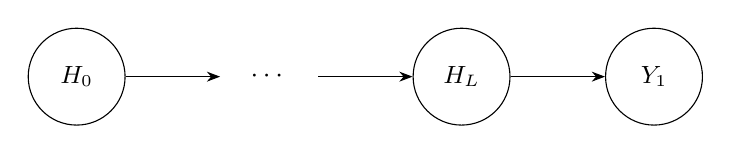
\begin{tikzpicture}[
      mycircle/.style={
         circle,
         draw=black,
         % fill=gray,
         fill opacity = 0.3,
         text opacity=1,
         inner sep=1pt,
         minimum size=35pt,
         font=\small},
      myarrow/.style={-Stealth},
      node distance=0.6cm and 1.2cm,
      node/.style={circle, draw, minimum size=35pt}
      ]
\node[mycircle            ] (y1) {$Y_1$};

\node[mycircle,left=of y1             ] (hL) {$H_{L}$};

\node[  circle,left=of hL             ,minimum size=35pt] (hl) {$\cdots$};

\node[mycircle,left=of hl             ] (h0) {$H_{0}$};

\foreach \i/\j in {% start node/end node
      hL/y1,hl/hL,h0/hl}
       \draw[myarrow] (\i) -- node {} (\j);

\end{tikzpicture}
\begin{minipage}{0.85\textwidth}
\caption{A directed acyclic graph depicting a deep Gaussian process with 
$L$ hidden layers. 
Each arrow represents a multivariate Gaussian process.
For deep GP regression, $H_0=X$.}
\end{minipage}
\label{fig:deepgp}
\end{figure}

\subsection{Deep GP with conditional independence amongst the nodes in a layer}


Following \cite{damianou2013deep},
a Deep GP (DGP) with $L$ hidden layers 
(note that $L=0$ is a regular GP) assumes
\begin{equation}
Y_d \ind GP_{\mathbb{R}^{D_{L}}}(m_{L,d},k_{L,d})
\label{eq:y}
\end{equation}
where $Y_d$ is the dimension $d$ output and $h_{L} \in \mathbb{R}^{D_{L}}$ is 
the input and
\begin{equation}
H_{\ell+1,d} \ind GP_{\mathbb{R}^{D_{\ell}}}(m_{\ell,d},k_{\ell,d})
\end{equation}
for $d=1,\ldots,D_{\ell}$ and $\ell = 0,\ldots,L-1$
where $H_{\ell,d}$ represents the dimension $d$ output and
$h_{\ell} \in \mathbb{R}^{D_{\ell}}$ are the inputs.
Each dimension output is independent of the others (conditional on the inputs),
but correlated (through $k_{\ell,d}$) within the dimension.





Figure \ref{fig:deepgp} presents a directed acyclic graphical representation
of this DGP which shows the DGP is \emph{fully connected} in the sense that all
dimensions of a hidden layer are available to each of the output dimensions
in the next hidden (or data) layer,
but the nodes within a layer are conditionally independent of each other.
% !TEX root = deepgp.tex

\begin{figure}[h]
\centering
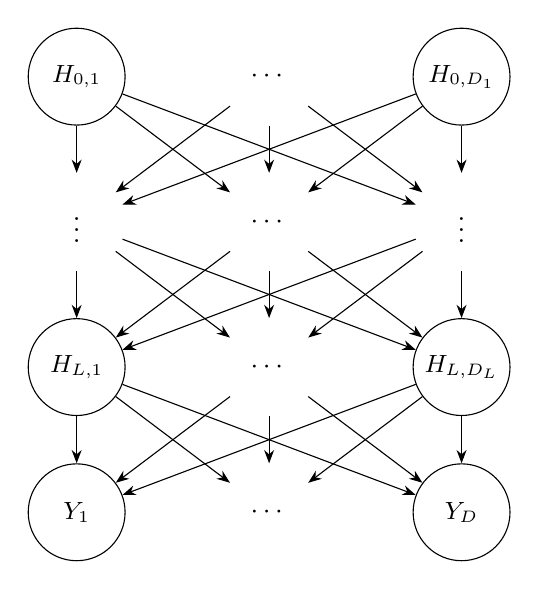
\begin{tikzpicture}[
      mycircle/.style={
         circle,
         draw=black,
         % fill=gray,
         fill opacity = 0.3,
         text opacity=1,
         inner sep=1pt,
         minimum size=35pt,
         font=\small},
      myarrow/.style={-Stealth},
      node distance=0.6cm and 1.2cm,
      node/.style={circle, draw, minimum size=35pt}
      ]
\node[mycircle            ] (y1) {$Y_1$};
\node[  circle,right=of y1,minimum size=35pt] (yd) {$\cdots$};
\node[mycircle,right=of yd] (yD) {$Y_D$};

\node[mycircle,above=of y1             ] (hL1) {$H_{L,1}$};
\node[  circle,above=of yd,right=of hL1,minimum size=35pt] (hLd) {$\cdots$};
\node[mycircle,above=of yD,right=of hLd] (hLD) {$H_{L,D_{L}}$};

\node[  circle,above=of hL1             ,minimum size=35pt] (hl1) {$\vdots$};
\node[  circle,above=of hLd,right=of hl1,minimum size=35pt] (hld) {$\cdots$};
\node[  circle,above=of hLD,right=of hld,minimum size=35pt] (hlD) {$\vdots$};

\node[mycircle,above=of hl1             ] (h01) {$H_{0,1}$};
\node[  circle,above=of hld,right=of h01,minimum size=35pt] (h0d) {$\cdots$};
\node[mycircle,above=of hlD,right=of h0d] (h0D) {$H_{0,D_1}$};

\foreach \i/\j in {% start node/end node
      hL1/y1, hL1/yd, hL1/yD,
      hLd/y1, hLd/yd, hLd/yD,
      hLD/y1, hLD/yd, hLD/yD,
      hl1/hL1,hl1/hLd,hl1/hLD,
      hld/hL1,hld/hLd,hld/hLD,
      hlD/hL1,hlD/hLd,hlD/hLD,
      h01/hl1,h01/hld,h01/hlD,
      h0d/hl1,h0d/hld,h0d/hlD,
      h0D/hl1,h0D/hld,h0D/hlD}
       \draw[myarrow] (\i) -- node {} (\j);

\end{tikzpicture}
\begin{minipage}{0.85\textwidth}
\caption{A directed acyclic graph depicting a deep Gaussian process with 
$L$ layers with conditional independences amongst the nodes within a layer. 
Each arrow represents a scalar Gaussian process.
For deep GP regression, $H_0=X$.}
\end{minipage}
\label{fig:deepgp}
\end{figure}








\subsection{Finite representation}

For $Y \in \mathbb{R}^{N \times D}$ and $X\in \mathbb{R}^{N\times Q}$
and letting $Y_d$ be the $d$th column of $Y$,
then we have
\[
Y_d \ind N(m_{L+1,d}, K_{L+1,d})
\]
where
\[
m_{L+1,d} = (m_{L+1,d}(h_{1,L},m_{L+1,d}(h_{N,L})^\top
\]

is the vector of values for the mean function evaluated at the output values for
hidden layer L, i.e. $h_{1,,1},\ldots,h_{1,,N}$ where
is the hidden layer 1 value associated with observation $n$, and
$K_{1,d}(h_1,h_1)$ is the covariance matrix with $n,n'$-element
$k_{1,d}(h_{1,n},h_{1,n'})$.


\subsection{Mean and covariance functions}

Since each arrow in Figure \ref{fig:deepgp} represents a GP,
we must select a mean and covariance function for each of these GPs.
\cite{damianou2013deep} chose the \underline{automatic relevance determination} (ARD)
kernel
\[
k_{\ell+1,d}(h,h') =
\sigma^2_{\ell,d} \exp\left(-\frac{1}{2} \sum_{d'=1}^{D_\ell} \omega_{\ell,d,d'} \left[ h_{d'} - h_{d'}' \right]^2\right)
\]
with parameters $\sigma^2_{\ell,d},\omega_{\ell,1},\ldots,\omega_{\ell,D_\ell} > 0$.
This kernel is anisotropic because the dimensions are given different weights
as determined by $\omega_{\ell,d}$.
If $\omega_{\ell,d} \approx 0$ (or at least much smaller than the remaining $\omega_{\ell}$,
then dimension $d$ in layer $\ell$ provides almost no contribution to the correlation between
observations.

\cite{dunlop2018deep} use a covariance function constructed following
\cite{paciorek2004nonstationary} who provide a general approach to constructing
nonstationary covariance kernels from stationary kernels.




\section{Inference}

\subsection{Model comparison}

Within the DGP framework,
we have the following model comparison issues:

\begin{itemize}
\item How many layers $L$ should there be?
\item What should the dimension be for layer $\ell$, $D_\ell$?
\end{itemize}
Ideally, we would use the marginal likelihood,
i.e. $p(y|L,D_1,\ldots,D_L)$, to help us decide how many layers there should be
and how many dimensions per layer.
Methods that aim at estimating the marginal likelihood,
e.g. through a variational lower bound on the marginal likelihood \citep{damianou2013deep},
could be used for model comparison purposes.

\subsection{Parameter estimation}

Suppose we have selected a given DGP with $L$ layers and $D_1,\ldots,D_L$
dimensions for layers $1$ to $L$ respectively.
This DGP has $M=\sum_{\ell=1}^L D_\ell$ individual GPs,
see Figure \ref{fig:deepgp}.

Each individual GP has a set of parameters defining its mean function $m$ and
covariance function $k$.


\appendix
\section{Multivariate normal properties}
\label{app:normal}

Let

\[
\left( \begin{array}{c} Y_1 \\ Y_2 \end{array} \right) \sim
n\left(\left[\begin{array}{c} \mu_1 \\ \mu_2 \end{array} \right] ,
\left[\begin{array}{cc} \Sigma_{1,1} & \Sigma_{1,2} \\
\Sigma_{2,1} & \Sigma_{2,2} \end{array} \right]\right)
\]

By properties of multivariate normals, we have

\[
Y_2|Y_1=y_1 \sim N\left(\mu_{2|1}, \Sigma_{2|1}\right)
\]
where
\[
\mu_{2|1} = \mu_2 + \Sigma_{2,1}\Sigma_{1,1}^{-1}(y_2-\mu_2)
\quad \mbox{and} \quad
\Sigma_{2|1} = \Sigma_{2,2} - \Sigma_{2,1}\Sigma_{1,1}^{-1}\Sigma_{1,2}.
\]

\subsection{Conditional distributions}

By properties of multivariate normals in Section \ref{app:normal},
we can derive the following conditional distributions:
\begin{itemize}
\item Observations $\tilde{Y}$ at locations $\tilde{x}$:
\[
\tilde{Y}|Y=y,m,k,x,\tilde{x} \sim N\left(\tilde{m},\tilde{K}\right)
\]
with
\[
\tilde{m} = m_{1:N} + K_{Y,\tilde{Y}}K_{\tilde{Y},\tilde{Y}}^{-1}(y-m_{1:N})
\quad \mbox{and} \quad
\tilde{K} = K_{\tilde{Y},\tilde{Y}} - K_{\tilde{Y},Y}K_{\tilde{Y},\tilde{Y}}^{-1}K_{\tilde{Y},Y}
\]
\end{itemize}


\bibliography{deepgp}

\end{document}
